%! Author = nail
%! Date = 9/11/20

\chapter{Proposed Approach}\label{ch:proposed-approach}
\chead{}
\lhead{\bfseries \chaptername {\,} \thechapter }
\cfoot{\bfseries \thepage}
\rhead{}
\rhead{\bfseries Proposed Approach}
\section{Introduction}\label{sec:introduction-ch3}
During the first chapter, we have seen the essentials of concepts and techniques
about the image, which we will use for the remainder of this paper. In the second
chapter, we presented the active contours, their characteristics, and their limits, and
it's descendant improvement model the GVF field which helps the snakes to have a
better capture range to the object boundaries, which also require a considerable
time for processing.\\
Parallelism is an effective way to speed up the convergence of the contour, serval
methods are proposed to optimize the time of computation by using parallel
computing. The initialization of the snake has an impact in processing time when the
initial snake contour is to closer to the object boundary the processing time it's
goanna be lower while when it's distant processing time increase.
In this chapter, we are going to define our proposed approach that help minimize the
computation time, First we are going to define another way of initialization for the
initial snake contour by using k-means clustering and Quick-hull algorithm, then we
apply parallel realization of the GVF snake.
Once the method has been defined, the most important phase is implementation.
This implementation will allow us to study the behavior of the method proposed
through a series of experiments test. So the second part of this chapter is assigned to
the experimental results of our work.
\section{GVF-Snake Parallel execution}\label{sec:gvf-snake-parallel-execution}
The steps of the proposed approach can be summarized as follows:

\begin{figure}[ht]
    \centering
    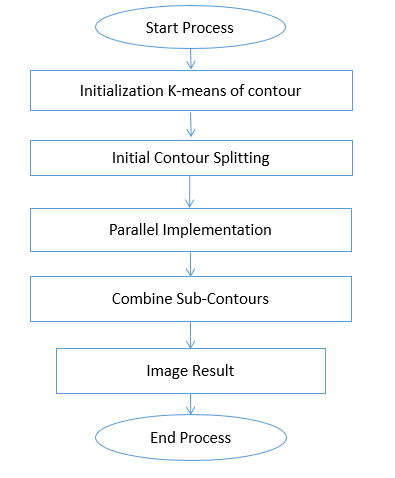
\includegraphics[width=12cm]{chapiter3/figures/figure 01 Approach Process.png}
    \setlength{\fboxrule}{2pt}
    \caption{Approach Process}
    \label{fig:figure3.1}
\end{figure}

\subsection{Snake Initialization}\label{subsec:snake-initialization}
As we see in the previous chapter, the snake has a problem of initialization and its
sensitivity to noise, so the initial contour is an influential factor of the result and the
computation time. In this section, we introduce another way to initialize the snake,
which gives us a closer initialization to the object boundary by using the K-means
clustering and quick hull algorithm. First, we will set some definitions about them,
and then we will explain the process of this approach.\\

\subsubsection{k-means clustering}
Currently, the clustering method often used for segmenting large-scale images
performs pre-treatment of images, which can be implemented with less complicated
clustering algorithm or others. In which a set of essentials is separated into uniform
groups, there are different types of clustering: K-means clustering, Fuzzy C-means
clustering, mountain clustering method, and subtractive clustering method. One of
the most used clustering algorithms is k-means clustering. It is simple and
computationally faster than the hierarchical clustering.

\subsubsection*{K-means Procedure}
K-means is an efficient clustering technique. Based on the initial centroids of the
cluster. Clustering is a method to divide a set of data into a specific number of
groups.\\
According to this algorithm, firstly we choose k as an initial number of cluster, then
assign each pixel to the nearest cluster, by calculating the difference between the
value of pixels and the center of each cluster.\\
Let us consider an image with a resolution of m*n and the image has to be cluster
into k number of clusters. Let $I(x, y)$ be an input pixel to be cluster. The algorithm for
k-means clustering is following as:
\begin{enumerate}
    \item Initialize number of cluster k.
    \item Calculate the Max and min value of pixel in image, which determine the
    interval value of the image.
    \item Divide image interval into k interval (classes), and initialize the centers of the
    class with the half of each interval.
    \item Assign all the pixels to the nearest class based on the difference between the
    center of class and pixel value (assign pixel to class where the difference is
    small).
    \item Reshape the cluster pixels into image.
\end{enumerate}
The application of the k-means algorithm in images divides the image into regions
(objects), and every region is a cluster, so we have the pixels of each cluster, and that
allows us to take a closer initialization to the object by identifying the points around
the object(Convex Hull).\\
In geometry, the convex hull or convex envelope or convex closure of a shape is the
smallest convex set that contains it. The convex hull may be defined either as the
intersection of all convex sets containing a given subset of Euclidean space, or
equivalently as the set of all convex combinations of points in the subset. For
a bounded subset of the plane, the convex hull may be visualized as the shape
enclosed by a rubber band stretched around the subset \cite{3.1}.\\
In computational geometry, numerous algorithms are proposed for computing
the convex hull of a finite set of points, with various computational complexities
like Chan's algorithm, Monotone chain, and Quick-hull .we choose a quick hull
algorithm, which introduced by C. Barber and D. Dobkin in 1995, It is efficient and
simple and easy to implement.
\subsubsection{Quick hull algorithm}
Quick-hull is a method of computing the convex hull of a finite set of points in the
plane. It uses a divide and conquer approach similar to that of quicksort, from which
its name derives. It is simple and easy to implement, and its average-case complexity
is considered to be O(n * log(n)) \cite{3.2}.
\subsubsection*{Quick Hull Procedure}
The Quick-Hull algorithm is a Divide and Conquer algorithm similar to Quick-Sort. Let
$a[0,\ldots, n-1]$ be the input array of points. Following are the steps for finding the convex
hull of these points \cite{3.3}.
\begin{enumerate}
    \item Find the point with minimum x-coordinate lets say, min-x and similarly the
    point with maximum x-coordinate, max-x ,see figure(\ref{fig:figure3.2}).
    \item Make a line joining these two points, say L. This line will divide the whole set
    into two parts. Take both the parts one by one and proceed further x,see figure(\ref{fig:figure3.2}).

    \begin{figure}[ht]
        \centering
        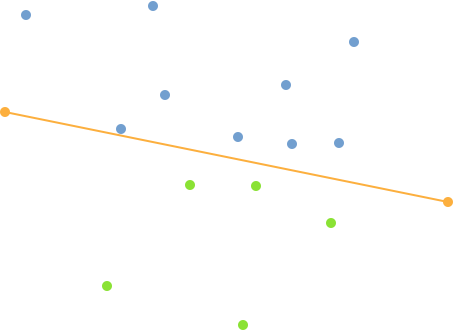
\includegraphics[width=12cm]{chapiter3/figures/figure 02 Steps 1-2 Divide points in two subsets.png}
        \setlength{\fboxrule}{2pt}
        \caption{Steps 1-2 Divide points in two subsets}
        \label{fig:figure3.2}
    \end{figure}
    \vspace{2cm}
    \item For a part, find the point P with maximum distance from the line L. P forms a
    triangle with the points min-x, max-x. It is clear that the points residing inside
    this triangle can never be the part of the convex hull as it show in figure(\ref{fig:figure3.3}) .
    \begin{figure}[ht!]
        \centering
        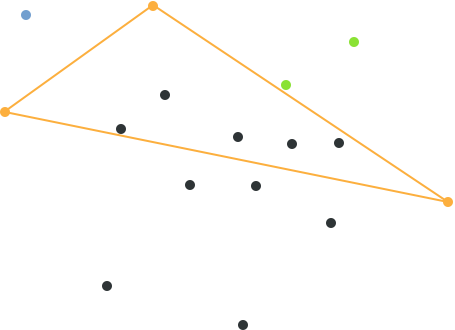
\includegraphics[width=12cm]{chapiter3/figures/FIG3.png}
        \setlength{\fboxrule}{2pt}
        \caption{Step 3 Find maximal distance point, ignore points inside triangle and repeat it}
        \label{fig:figure3.3}
    \end{figure}

    \item The above step divides the problem into two sub-problems (solved
    recursively). Now the line joining the points P and $min_x$ and the line joining
    the points P and $max_x$ are new lines and the points residing outside the
    triangle are the set of points. Repeat until there no point left with the line. Add
    the endpoints of this point to the convex hull, see figure(\ref{fig:figure3.4}).\\
    \begin{figure}[ht!]
        \centering
        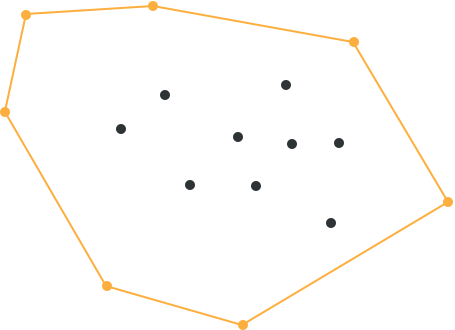
\includegraphics[width=12cm]{chapiter3/figures/figure 04 3 Recourse until no more points are left.png}
        \setlength{\fboxrule}{2pt}
        \caption{3 Recourse until no more points are left}
        \label{fig:figure3.4}
    \end{figure}

\end{enumerate}

\subsubsection{Initialization Process}
The Process of our initialization method begins by converting the image I to grayscale
image. Then to begin our process, which includes two steps, these steps can be
summarized as follows:
\begin{itemize}
    \item The first step is applying the k-means algorithm in the grayscale image I, with k
    cluster, which will divide the image into regions (objects) and extract our
    cluster which represent our object.
    \item The second step is to define the points surrounding the cluster (object) by
    applying Quick Hull algorithm ,which gives us a set of points that represent our
    initial contour.
\end{itemize}

\subsection{Initial Contour Splitting}\label{subsec:initial-contour-splitting}
For the active contour algorithm to find the objectboundaries, an initial contour
needs to be defined first which we have it from the above step. Asthe initial contour
is define , the region where the objectlies in is determined, and we call this region
our Regionof Interest (ROI). In our approach Instead of subdividing the image, wesplit
the contour into two sub-contours.\\
After the initial contour is drawn, its four coordinatesis selected, including the
most left, top, right and bottomposition $(leftX, rightX,topY,bottomY)$.With these four
parameters, two points $P_{start}$, $P_{end}$ are created,where $P_{start} = (leftX , topY + (bottomY -
topY )/2)$ and $P_{end} = (rightX, topY + (bottomY - topY )/2)$.
Then we creating ablack line from $P_{start}$ to $P_{end}$.
as a result,the contour is split into two sub-contours with similarsize.
In order to make the sub-contours converge to the object boundary, they
must be end to form a loop,so we used the black line as part of the two sub
contoursto help them to form a loop.\\
Now we need to get the points of the two sub-contours so that to compute their
energies and to converge. According to the positions of $P_{start}$ and $P_{end}$ , we can find the
nearest points from the black line as the cutting points, then the points of the contour
are divided into two sets with each set belong into one sub-contour, and by adding
the points from the black line with equal distance, we finally get two sub-contours.

\subsection{Parallel Implementation}\label{subsec:parallel-implementation}
The initial contour is now divided into two sub-contours,which are independent from
each other. Then the two sub-contours can converge in parallel. The object on the
image is also divided into two sub-objects by the black line.On each sub-contour,
thepoints move to the sub-object boundary iteratively. For the points on the black
line, because wetake the black line as the imaginary boundary of thesub-object,
which means that they are already on the boundary, so in our method, we do not
move these pointsat all to save the convergence time.\\
We implement the parallelism by $Java$ multi-thread on a multi core platform.Each sub-
contour is assigned to one thread, which then runs in parallel to converge towards the
object boundary.
\subsection{Combine Sub-Contours into the Whole Contour}\label{subsec:combine-sub-contours-into-the-whole-contour}
With the two converged sub-contours, we can get the whole contour of the object by
combining them together.\\
First, we delete the points of the two sub-contours which the black line are they
boundary because as mentioned before we take the black line as imagery-boundary .
After that, we get just the points of the two sub-contour and we can combine them
together to get the whole contour. For the deleting of the black line, we just remove
the image split with the black-line and replace it by the original image.
Finally, we display the whole contour on the image.

\section{Snake Evolution}\label{sec:snake-evolution}
\subsection{Energy}\label{subsec:energy}
We remind that the snake consists of placing around the shape to detect an initial
contour line. This line will gradually deform and move under the influence of several
forces that will pull it or push it towards the object. The forces involved will derive
three energies associated with the snake. The functional energy attached to the snake is:

\begin{equation}
    E(C) = \alpha E_{tinuity} + \beta E_{curvature} + \gamma E_{Gvf}
    \label{eq:eq3.1}
\end{equation}


\hspace{-0.6cm}Each terms corresponds to a particular type of force, we have introduced three-term
energy that must be minimized along the contour, so the evolution of the contour is
obtained by minimization of this functional.

\subsubsection{Continuity Energy}
The energy $E_{con}(s_{i})$ is defined for any point in the Snake as the value absolute of the
difference between two distances, the average distance between points $\bar{d}$
(calculated for each iteration) and the distance between the previous point $s_{i-1}$
contour and point $s_{i}$ :

\begin{equation}
    E_{con}(s_i) = \bar{d} - \| v(s_i) - v(s_{i-1}) \| = \bar{d} - \sqrt{(x(s_i) - x(s_{i-1}) - 1)^2 + (y(s_i) - y(s_{i-1}) - 1)^2}
    \label{eq:eq3.2}
\end{equation}

\subsubsection{Curvature Energy}
The curvature energy is calculated as the following equation:
\begin{equation}
    E_{cur}(s_i) = ( x(s_{i-1}) + x(s_i) + x(s_{i+1}) )^2 + ( y(s_{i-1}) + y(s_i) + y(s_{i+1}) )^2
    \label{eq:eq3.3}
\end{equation}

\subsubsection{GVF Field}
The GVF field is calculated in the beginning by calculating U and V as we explained in
the chapter(\ref{ch:active-contours-:-gvf-snakes}),each pixel or cell of the image matrix
will be calculated according to its neighbors weighted.

\subsection{Energy Minimization}\label{subsec:energy-minimization}
To solve the problem of minimization of the functional energies, we use the Greedy
algorithm (described in the second chapter); the algorithm is iterative, which move a
single point in the neighborhood $(size :3*3)$ to constitute a new active contour at
each iteration ,figure(\ref{fig:figure3.5}) represent an organigramme describe greedy process .

\begin{figure}[ht!]
    \centering
    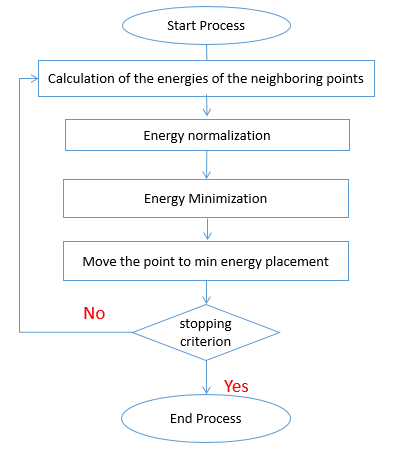
\includegraphics[width=12cm]{chapiter3/figures/Figure 5 Greedy Process.png}
    \setlength{\fboxrule}{2pt}
    \caption{Greedy Process}
    \label{fig:figure3.5}
\end{figure}

\hspace{-0.6cm}The snake stops by checking a stop criterion, which is related with the number of
iterations achieved or no .

\section{Hardware and Software environment}\label{sec:hardware-and-software-environment}
In order to verify the effectiveness of the proposed approach, we used machine type
Intel i7-6500U with 2.50 GHz frequency processor, a RAM of 8GB, and a 240 GB SSD
drive. The machine runs under the environment Linux.\\
We have use JavaFx programming language, for the many tools it offers for fast and
efficient development of applications and including ease of handling images and files.
\vspace{4cm}
\section{Results and Experiment}\label{sec:results-and-experiment}
To study the performance of the proposed approach, we used three image, which
contain deferent object in it: elliptical, concave and ellipsoid.\\
We will present the application of each step of our process then we will do a
comparison in Object Detection and Tracking and in the computation time of our
snake with our approach and in the normal case .

\subsection{Approach Process application}\label{subsec:approach-process-application}
\subsubsection{Snake Initialization with K-means}
The figure(\ref{fig:figure3.6}) show us the application of k-means in image, as we can see its give us a
closer initialization to object Boundaries.

\begin{figure}[ht!]
    \centering
    \begin{subfigure}[b]{1\textwidth}
        \centering
        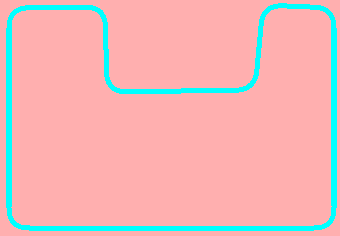
\includegraphics[width=12cm,height=8cm]{chapiter3/figures/k-means-region.png}
        \caption{K-means algorithm}
    \end{subfigure}
    \hfill
    \begin{subfigure}[b]{1\textwidth}
        \centering
        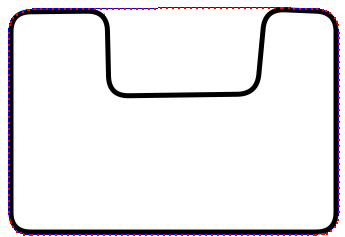
\includegraphics[width=12cm,height=8cm]{chapiter3/figures/figure 06 initilization using k-means.png}
        \caption{Quick-hull algorithm}
    \end{subfigure}
    \caption{auto initialization of contour}
    \label{fig:figure3.6}
\end{figure}

\subsubsection{Initial Contour Splitting}
In this step wesplit the contour into two sub-contours which are independents to
each other ,see figure(\ref{fig:figure3.7}).

\begin{figure}[ht!]
    \centering
    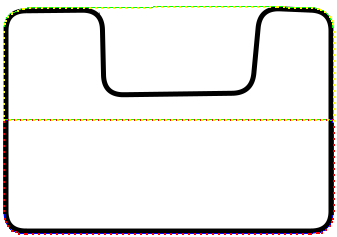
\includegraphics[width=12cm,height=8cm]{chapiter3/figures/figure 11 b.png}
    \setlength{\fboxrule}{2pt}
    \caption{Splitting initial contour}
    \label{fig:figure3.7}
\end{figure}

\subsubsection{Parallel Implementation}
The two sub-contours will execute at the same time, each sub-contour is assigned to
one thread, which then runs in parallel to converge towards the object boundary. As
it's shown in figure(\ref{fig:figure3.8}), the result of the convergence of each sub-contour .

\begin{figure}[H]
    \centering
    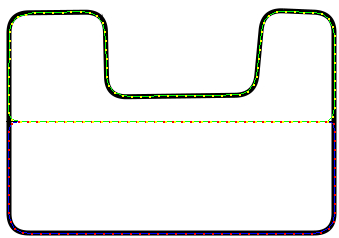
\includegraphics[width=12cm,height=7cm]{chapiter3/figures/FIG7.png}
    \setlength{\fboxrule}{2pt}
    \caption{Parallel execution of the two sub-contour}
    \label{fig:figure3.8}
\end{figure}

\subsubsection{Combine Sub-Contours into the Whole Contour}
As we see in the previous step, we got tow converged sub-contours, so now we
combine them to get the whole contour of the object, see figure(\ref{fig:figure3.9}).

\begin{figure}[H]
    \centering
    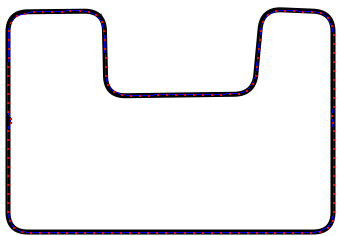
\includegraphics[width=12cm,height=8cm]{chapiter3/figures/figure 09.png}
    \setlength{\fboxrule}{2pt}
    \caption{Whole Contour}
    \label{fig:figure3.9}
\end{figure}

\subsection{Result of our Approach}\label{subsec:result-of-our-approach}
We will select and display the object detection and tracking results in three
images,which contain three different shapes as we said.\\
The coefficient of the energy $\alpha$, $\beta$ and $\gamma$ having the same value in this result
$\alpha = \beta = \gamma = 1$

\subsubsection{Concave Shape}

\textbf{Snake parameter}

\begin{table}[H]
    \begin{tabular}{ |p{2cm}|p{2cm}|p{2cm}|p{2cm}|p{2cm}|p{2cm}| }
        \hline
        \multicolumn{3}{|c|}{Sub-contour 01} & \multicolumn{3}{|c|}{Sub-contour 02} \\
        \hline
        Nb points of initial contour &
        Nb points of final contour &
        Nb points of iteration &
        Nb points of initial contour &
        Nb points of final contour &
        Nb points of iteration
        \\
        \hline
        149   &  95    &  3 & 149  & 108  & 273 \\

        \hline
    \end{tabular}
    \caption{Snake parameter of Concave Shape}
    \label{tab:table01}
\end{table}


\begin{figure}[H]
    \centering
    \begin{subfigure}[b]{1\textwidth}
        \centering
        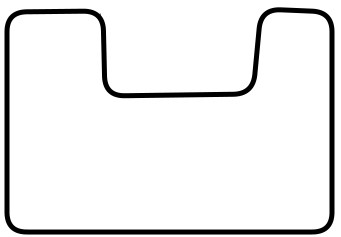
\includegraphics[width=12cm,height=6.5cm]{chapiter3/figures/Figure 11 a.jpg}
        \caption{Original image}
    \end{subfigure}
    \hfill
    \begin{subfigure}[b]{1\textwidth}
        \centering
        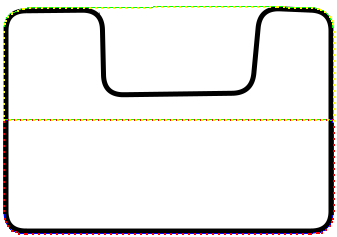
\includegraphics[width=12cm,height=6.5cm]{chapiter3/figures/figure 11 b.png}
        \caption{Initialization}
    \end{subfigure}
    \hfill
    \begin{subfigure}[b]{1\textwidth}
        \centering
        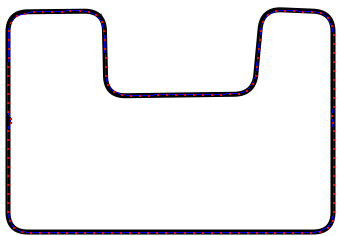
\includegraphics[width=12cm,height=6.5cm]{chapiter3/figures/figure 09.png}
        \caption{Result}
    \end{subfigure}
    \caption{result of approche in Concave Shape}
    \label{fig:figure3.10}
\end{figure}

\subsubsection{heart Shape}

\textbf{Snake parameter}

\begin{table}[H]
    \begin{tabular}{ |p{2cm}|p{2cm}|p{2cm}|p{2cm}|p{2cm}|p{2cm}| }
        \hline
        \multicolumn{3}{|c|}{Sub-contour 01} & \multicolumn{3}{|c|}{Sub-contour 02} \\
        \hline
        Nb points of initial contour &
        Nb points of final contour &
        Nb points of iteration &
        Nb points of initial contour &
        Nb points of final contour &
        Nb points of iteration
        \\
        \hline
        130   &  78    &  17  & 130  & 95  & 42 \\

        \hline

    \end{tabular}
    \caption{Snake parameter of heart Shape}
    \label{tab:table02}
\end{table}


\begin{figure}[H]
    \centering
    \begin{subfigure}[b]{1\textwidth}
        \centering
        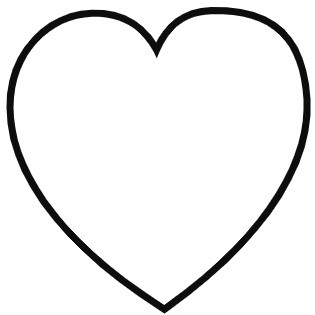
\includegraphics[width=12cm,height=9cm]{chapiter3/figures/figure 12 a.jpeg}
        \caption{Original image}
    \end{subfigure}
    \caption{result of approche in Heart Shape}
    \label{fig:figure3.11}
\end{figure}
\begin{figure}[H]\ContinuedFloat
    \begin{subfigure}[b]{1\textwidth}
        \centering
        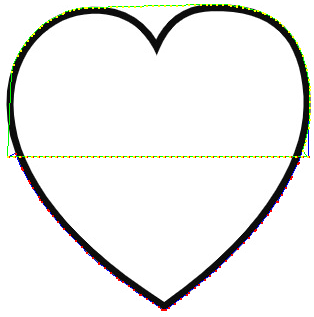
\includegraphics[width=12cm,height=9cm]{chapiter3/figures/figure 12 b.png}
        \caption{Initialization}
    \end{subfigure}
    \hfill
    \begin{subfigure}[b]{1\textwidth}
        \centering
        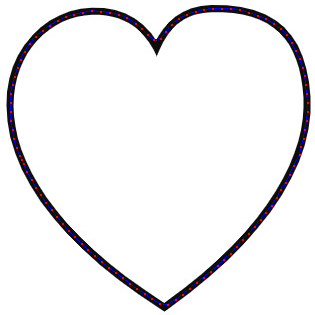
\includegraphics[width=12cm,height=9cm]{chapiter3/figures/figure 12 c.png}
        \caption{Result}
    \end{subfigure}
    \caption{result of approche in Heart Shape}
    \label{fig:figure3.11.1}
\end{figure}
\vspace{2cm}
\subsubsection{Ellipsoid Shape}

\textbf{Snake parameter}

\begin{table}[H]
    \begin{tabular}{ |p{2cm}|p{2cm}|p{2cm}|p{2cm}|p{2cm}|p{2cm}| }
        \hline
        \multicolumn{3}{|c|}{Sub-contour 01} & \multicolumn{3}{|c|}{Sub-contour 02} \\
        \hline
        Nb points of initial contour &
        Nb points of final contour &
        Nb points of iteration &
        Nb points of initial contour &
        Nb points of final contour &
        Nb points of iteration
        \\
        \hline
        100   &  77    &  11  & 101  & 103  & 90 \\

        \hline
    \end{tabular}
    \caption{Snake parameter of Ellipsoid Shape}
    \label{tab:table03}
\end{table}


\begin{figure}[H]
    \centering
    \begin{subfigure}[b]{1\textwidth}
        \centering
        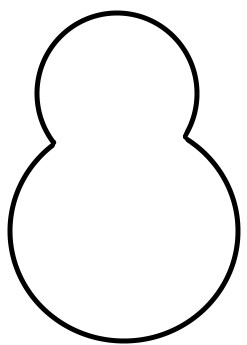
\includegraphics[width=12cm,height=9cm]{chapiter3/figures/figure 13 a.jpg}
        \caption{Original image}
    \end{subfigure}
    \caption{result of approche in Ellipsoid Shape}
    \label{fig:figure3.12}
\end{figure}
\begin{figure}[H]\ContinuedFloat
    \begin{subfigure}[b]{1\textwidth}
        \centering
        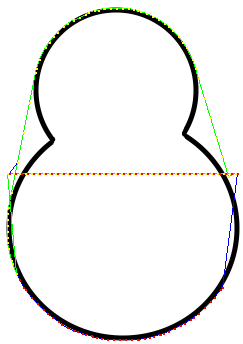
\includegraphics[width=12cm,height=8cm]{chapiter3/figures/figure 13 b.png}
        \caption{Initialization}
    \end{subfigure}
    \hfill
    \begin{subfigure}[b]{1\textwidth}
        \centering
        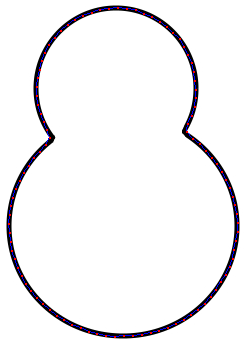
\includegraphics[width=12cm,height=8cm]{chapiter3/figures/figure 13 c.png}
        \caption{Result}
    \end{subfigure}
    \caption{result of approche in Ellipsoid Shape}
    \label{fig:figure3.12.1}
\end{figure}

\hspace{-0.6cm}As we can see in the figure (\ref{fig:figure3.10}),(\ref{fig:figure3.11}),(\ref{fig:figure3.12}) 
we note that the object boundary is well
detected in all image and that's up to the closer initialization and the parallel
implementation of the contour because it reduces the number of iteration so in
terms of performance and detecting object its give us a perfect result. In the next
section, we are going to see the impact of it in term of the computation time.

\subsection{Comparison time}\label{subsec:comparison-time}
A temporal comparison was based on four methods:
\begin{enumerate}
    \item normal GVF
    \item our approach: k-means and the parallel implementation
\end{enumerate}
The comparison is summarized in Table(\ref{tab:table04}):\\

\begin{table}[H]
    \centering
    \begin{tabular}{ |c|c|c|c| }
        \hline
        \textbf{Shape} &  \textbf{Normal GVF} & \multicolumn{2}{|c|}{\textbf{Proposed approach}} \\
        \hline
        & whole contour  & sub-contour 01  & sub-contour 02 \\
        \hline
        Heart & 140 & 2 & 4 \\
        \hline
        Concave & 525 & 2 & 17 \\
        \hline
        Ellipsoid & 138 & 1 & 7 \\

        \hline
    \end{tabular}
    \caption{Comparison of method in the computation time in ms}
    \label{tab:table04}
\end{table}

\hspace{-0.6cm}The table (\ref{tab:table04}) show us the main result of our method by comparing
the time of the normal GVF and our approach. we noting that
the time in the parallel implementation is taking from the sub-contour which have
large value because they run in parallel like in the Heart shape we got 2 form sub-
contour one and 4 form sub-contour two ,so the total time is 4.

\section{Conclusion}\label{sec:conclusion}

In this chapter, we have presented our method of parallelism the GVF snack.Its
approach parallel, which initialize the first contour by the k-means clustering
algorithm and get the points of contour by Quick-hell algorithm then splitting that
contour to two sub-contour, which converge to the object boundaries in parallel due
of multi-core platform.\\
The experiments were carried out on three images. The results obtained show
thatthe major advantage of our approach is the minimization of the detection time
of the object .We can see that our approach reduce over than 90% in computation
time compared tothe normal GVF-Snack and give better result than the other
method.